\documentclass[a4paper,10pt]{article}
\usepackage[utf8]{inputenc}
\usepackage{amsmath}
\usepackage{xfrac}
\usepackage{float}
\usepackage[a4paper, total={7.5in, 10in}]{geometry}
\usepackage{longtable}
\usepackage{dcolumn,booktabs}
\usepackage[table]{xcolor}
\usepackage{listings}
\lstset{
breaklines=true
}
%http://tex.stackexchange.com/questions/116534/lstlisting-line-wrapping
\usepackage{hyperref}
\hypersetup{
    colorlinks=true,
    linkcolor=blue,
    citecolor=blue
}

\lstset{language=[77]Fortran,
  basicstyle=\ttfamily,
  keywordstyle=\color{red},
  commentstyle=\color{green},
  morecomment=[l]{!\ }% Comment only with space after !
}

\usepackage{color}
 
\definecolor{codegreen}{rgb}{0,0.6,0}
\definecolor{codegray}{rgb}{0.5,0.5,0.5}
\definecolor{codepurple}{rgb}{0.58,0,0.82}
\definecolor{backcolour}{rgb}{0.95,0.95,0.92}
 
\lstdefinestyle{mystyle}{
    backgroundcolor=\color{backcolour},   
    commentstyle=\color{codegreen},
    keywordstyle=\color{magenta},
    numberstyle=\tiny\color{codegray},
    stringstyle=\color{codepurple},
    basicstyle=\footnotesize,
    breakatwhitespace=false,         
    breaklines=true,                 
    captionpos=b,                    
    keepspaces=true,                 
    numbers=left,                    
    numbersep=5pt,                  
    showspaces=false,                
    showstringspaces=false,
    showtabs=false,                  
    tabsize=2
}
 
\lstset{style=mystyle}

%opening

\title{Homework 4 \\
\textbf{Harmonic and Anharmonic Oscillator}}
\author{Arvind Balasubramanian}
\date{}

\begin{document}
\maketitle
\section*{Python code and analysis}
\begin{lstlisting}[language=python]
import numpy as np
import cmath as c

def aofx(x,k,alpha):
    """
    Returns the function that equals d^2x/dt^2
    """
    return -k*(x**alpha)

def euler_cromer(x0, t0, t, delta_t, k, alpha):
    """
    Returns an array of x values from time t = t0 to t = t
    """
    t_array = np.arange(t0, t + delta_t, delta_t)
    x_array = np.zeros(len(t_array))
    v_array = np.zeros(len(t_array))
    x_array[0] = x0

    for i in range(1, len(t_array)):
        v_array[i] = v_array[i-1] + delta_t*aofx(x_array[i-1],k,alpha)
        x_array[i] = x_array[i-1] + delta_t*v_array[i]

    return t_array, x_array, v_array

def FourierTransform(t_array, f_array, w_ini, w_fin):
    """
    Function to calculate fourier transform (to calculate time period of oscillation)
    """
    w_array = np.linspace(w_ini, w_fin, 1000)
    f_of_w = np.zeros(len(w_array))
    for wi in range(len(w_array)):
        integral = 0
        for ti in range(len(t_array)):
            f1 = f_array[ti]*(c.exp(-1j*w_array[wi]*t_array[ti]))
            integral = integral + f1/np.sqrt(2.0*np.pi)
        f_of_w[wi] = integral

    return w_array, f_of_w
    
# Initial conditions        

x01 = 0.2 # amplitude
t0 = 0.0 # start time
delta_t = 0.1 # time step
t = 10.0 # end time

t_array1, x_array1, v_array1 = euler_cromer(x01, t0, t, delta_t, k, alpha)
w_array1, f_of_w1 = FourierTransform(t_array1, x_array1, wi, wf)
w_sel = w_array1[np.where(f_of_w1 == max(f_of_w1))[0][1]]
T_period = 2.0*np.pi/w_sel ### Time period of oscillation

\end{lstlisting}

The time period was obtained by getting a fourier transform of the obtained motion. The obtained values are shown below :

\begin{center}
 \begin{longtable}{||c||c|c|c||c|c|c||}
 \hline
 & \multicolumn{3}{c||}{Harmonic Oscillator} & \multicolumn{3}{c||}{Anharmonic Oscillator} \\
 \hline
 Amplitude (m) & 0.2 & 0.5 & 1.0 & 0.2 & 0.5 & 1.0\\
 \hline
 Time Period (s)_& 6.22 & 6.22 & 6.22 & 37.00 & 14.82 & 7.40 \\
 \hline
 \end{longtable}
\end{center}

\section*{Plotting the motion for both harmonic and anharmonic oscillator}
\begin{figure}[H]
\centering
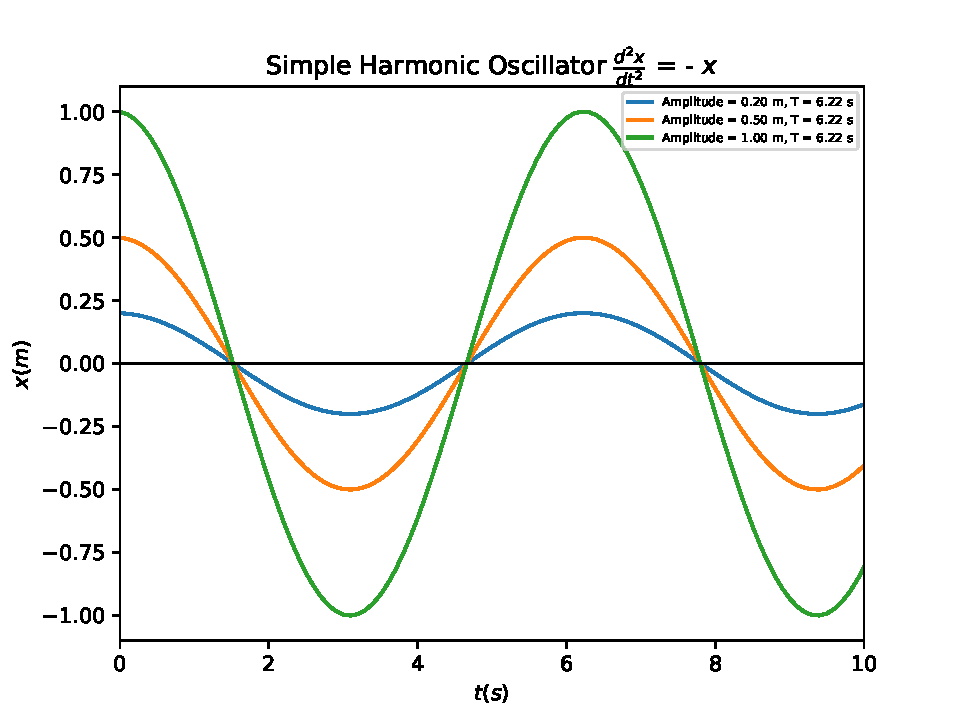
\includegraphics[scale=0.9]{harmonic_oscillator.pdf} 
\end{figure}

\begin{figure}[H]
\centering
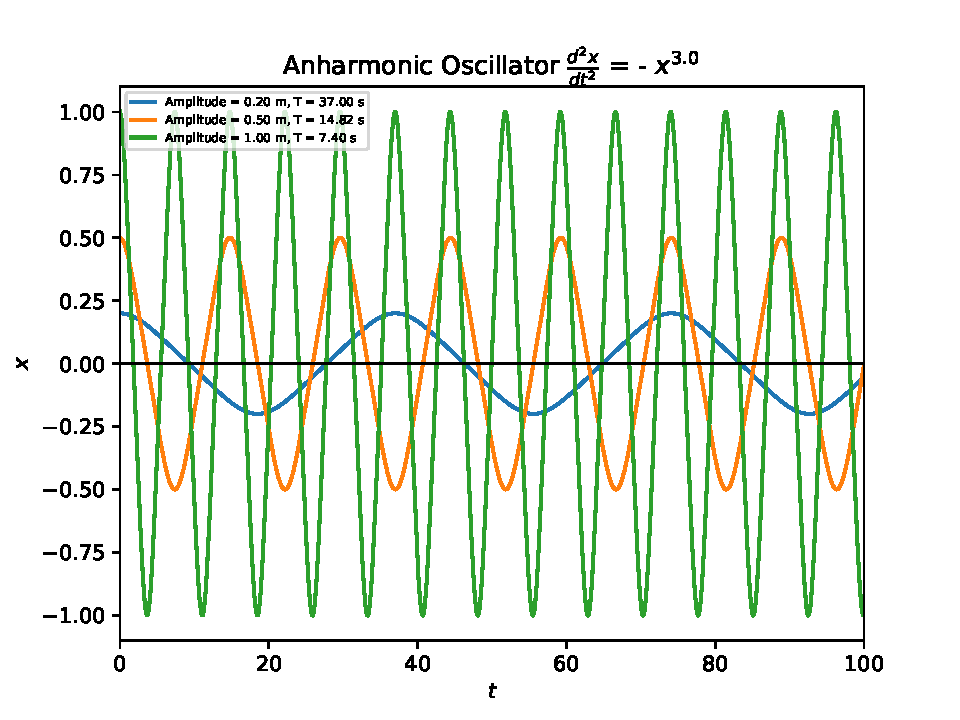
\includegraphics[scale=0.9]{anharmonic_oscillator.pdf} 
\end{figure}


\end{document}
